\documentclass[10pt]{article}
\usepackage[margin=0.72in]{geometry}
\usepackage{graphicx}
\usepackage{booktabs}
\usepackage{tabularx}
\usepackage{xcolor}
\usepackage[T1]{fontenc}
\usepackage{microtype}
\setlength{\parindent}{0pt}
\setlength{\parskip}{5pt}
\newcommand{\code}[1]{\texttt{#1}}
\begin{document}
\begin{center}
  {\LARGE\bfseries N6 formal proof-boundary report}\\[4pt]
  {\small Partial mechanization \textbullet{} generated 2026-10-25 \\
  Schema: \code{projective-law-formal-report/v1}}
\end{center}

\section*{Recorded result}
Lean 4.34.1 with pinned Mathlib revision
\code{d13f23b723b8a846827a245b89c10fc7d3f11612} kernel-checks three
branch-selection lemmas, three literal formula identities, totality of a
manual 17-row reachable-branch mapping, and application of an explicitly
caller-supplied divisor-class bridge. The formula identities include exact
factorizations for both generic 2+2 interpolation congruences.

The packet does not establish Rust-to-Lean semantic correspondence, a smooth
genus-2 curve or Mumford representation in Lean, the principal-divisor and
Picard-group bridge, complete exceptional-branch composition, or independent
mathematical review. The conditional bridge theorem constructs no bridge and
assumes no bridge globally.

\begin{center}
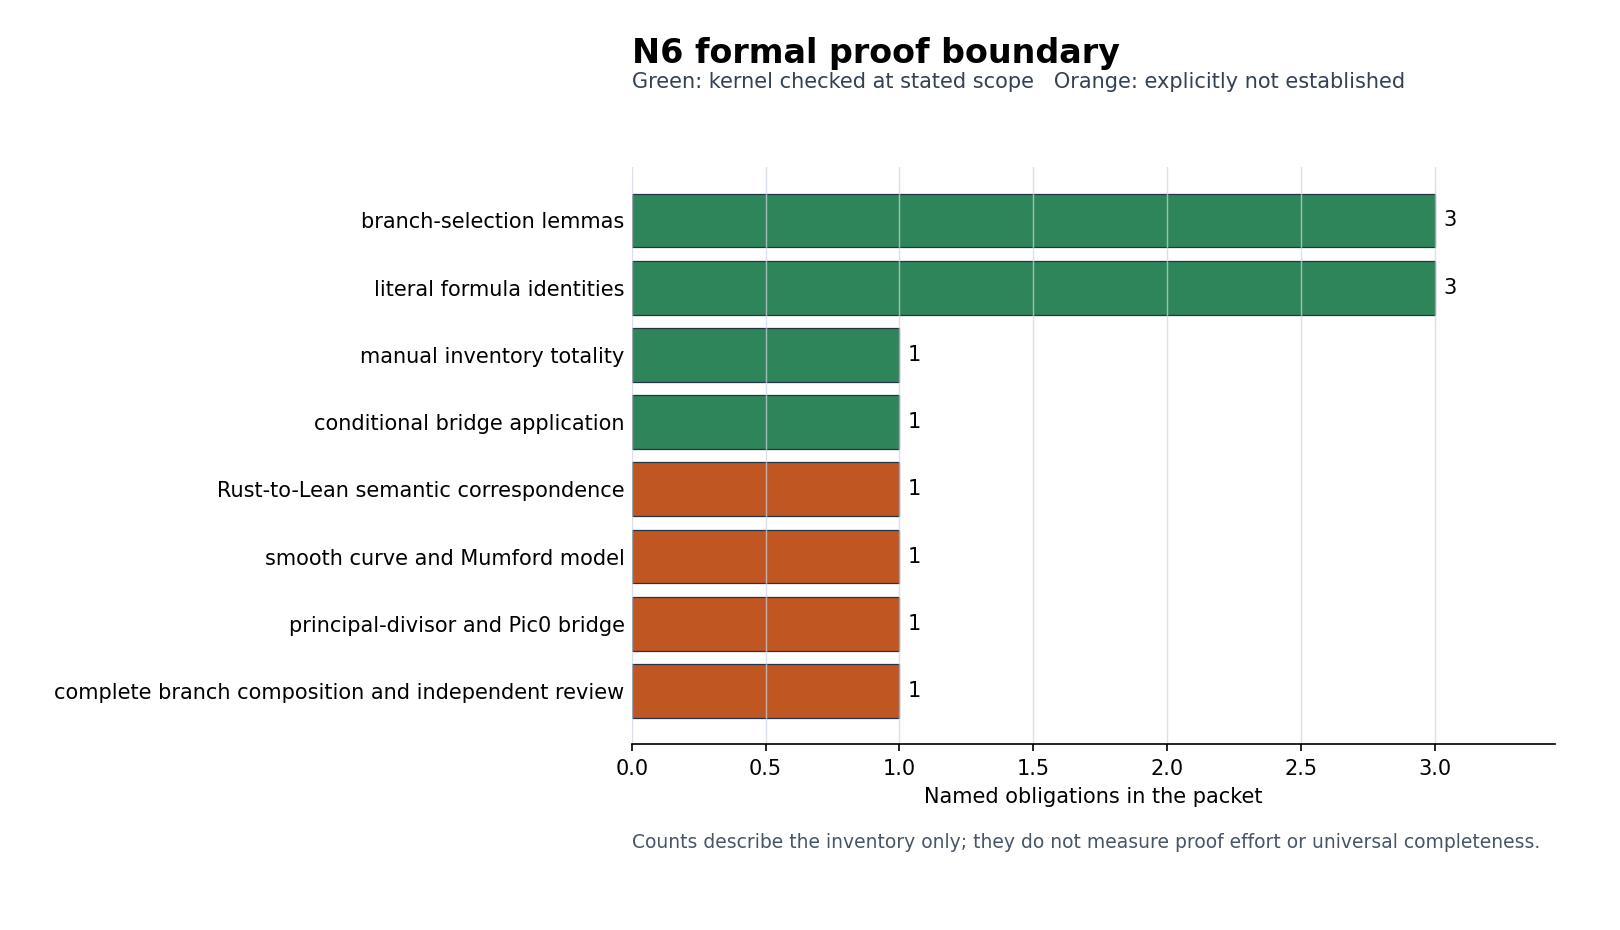
\includegraphics[width=0.94\textwidth]{formal-status.png}
\end{center}
\textit{Counts are an inventory of named obligations. They do not measure
proof effort, importance, or universal coverage.}

\section*{Standardized source table}
\small
\begin{tabularx}{\textwidth}{@{}p{0.28\textwidth}p{0.20\textwidth}X@{}}
\toprule
Evidence & Status & Scope or limit \\
\midrule
Three branch lemmas & Kernel checked & Abstract-field implications with explicit hypotheses. \\
Generic 1+2 identity & Kernel checked & Literal commutative-ring identity; no divisor argument. \\
Two generic 2+2 identities & Kernel checked & Exact factorizations by explicit input quadratics. \\
Runtime mapping & Kernel checked, manual scope & Total over a manually transcribed 17-row inventory; Rust is hash-bound, not parsed by Lean. \\
Conditional bridge & Kernel checked, conditional & Applies a caller-supplied implication; supplies no geometric bridge. \\
Source bindings & Integrity checked & Runtime, written audit, and eight native certificate source/result pairs are SHA-256 bound. \\
\bottomrule
\end{tabularx}
\normalsize

\section*{Validation and remaining boundary}
The cached rebuild completed 740 jobs. The axiom audit found only subsets of
\code{propext}, \code{Classical.choice}, and \code{Quot.sound}. The packet
verifier and SHA-256 manifest passed.

The next obligation is a faithful formal model joining the hashed Rust case
split to reduced Mumford divisor classes on the stated smooth quintic family,
including exceptional compositions and degree drops. Until that bridge is
supplied and independently reviewed, this packet records algebraic sublemmas
and a manual inventory rather than a universal group-law proof.
\end{document}
